% NeuroCam manual - GUI
% Written by Christopher Thomas.
% Copyright (c) 2021 by Vanderbilt University. This work is released under
% the Creative Commons Attribution-ShareAlike 4.0 International License.

\chapter{Web Interface}
\label{gui}

The NeuroCam system has three interface screens: The \textbf{configuration}
screen, the \textbf{monitoring} screen, and the \textbf{repository browser}.
The monitoring screen is seen when the system is collecting data. When the
system is not collecting data, the configuration screen and the repository
browser are both available.

\textbf{Important:} Do not use the ``back'' button of your web browser to
switch pages. This will result in stale CGI information being submitted.
Use the navigation buttons in the NeuroCam application instead.

\section{Configuration Screen}
\label{gui-config}

\begin{figure}[h]
\begin{center}
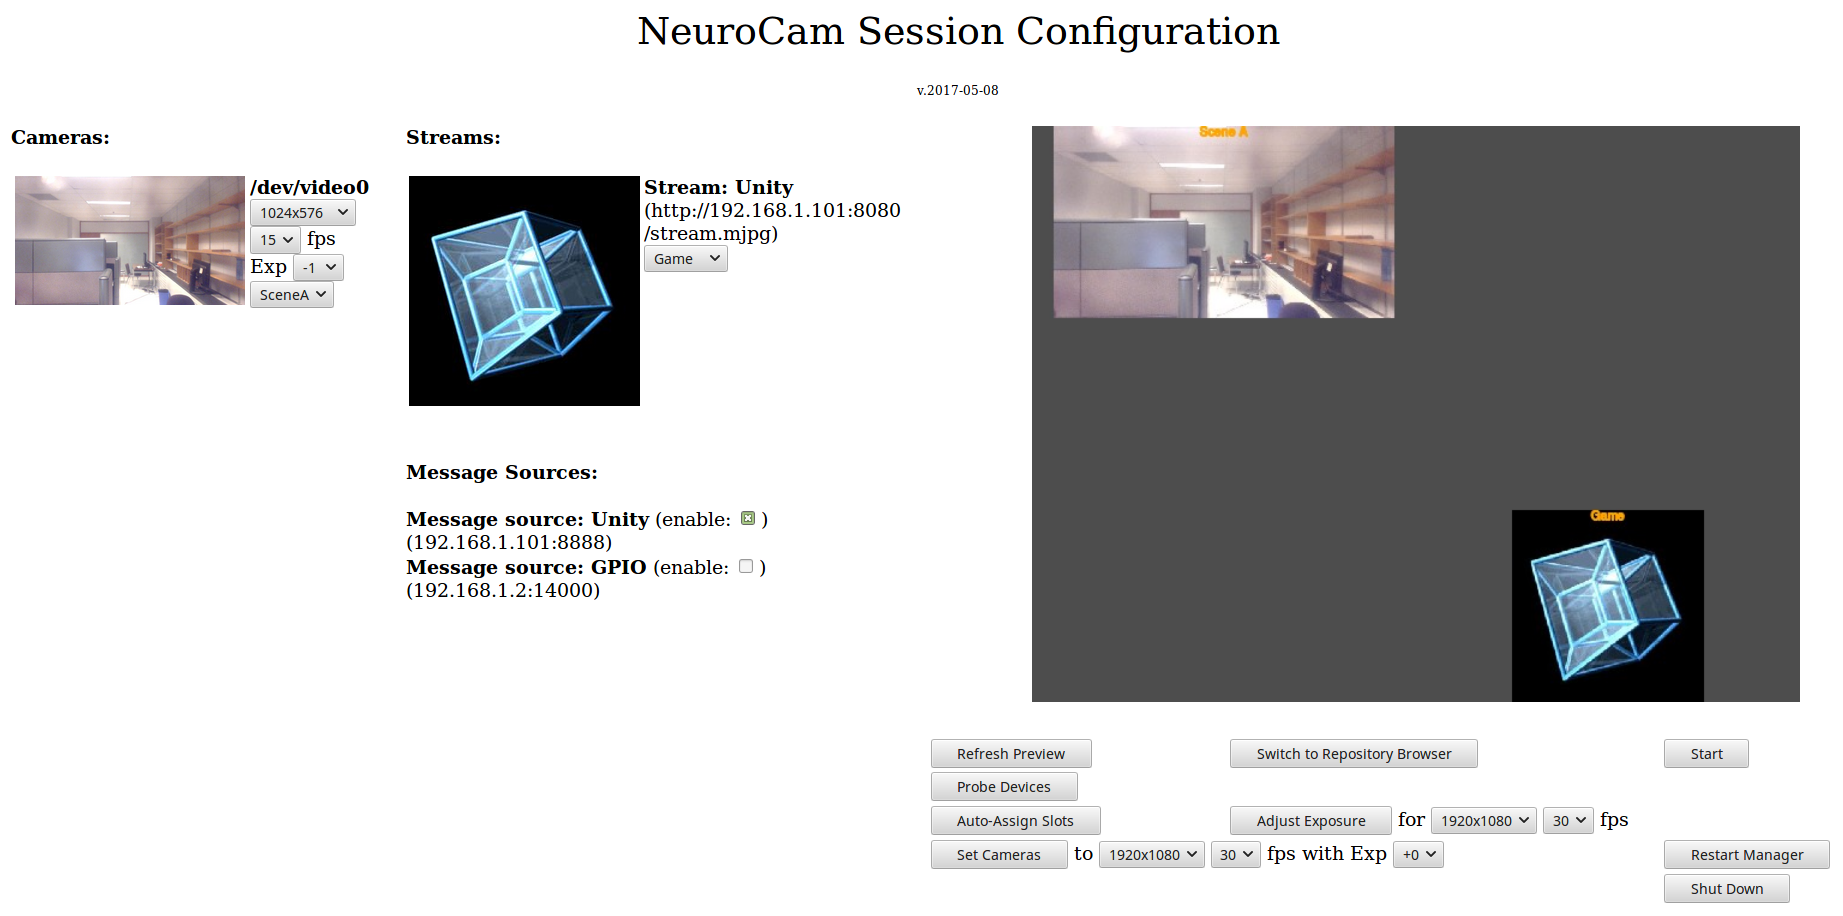
\includegraphics[width=0.95\textwidth]{pics-gui/gui-config.png}
\end{center}
\caption{Configuration screen.}\label{fig-gui-config}
\end{figure}

% FIXME - Annotate the image.

The configuration screen is used to set up a new video capture session.

Detected cameras are shown in the left column. The middle column shows
detected computer video streams and detected event message sources. The
right column shows a still-frame preview of the video feeds, with a control
panel under the preview.

Each camera has resolution, frame rate, and exposure settings, along with a
still-frame preview of its input. Longer (positive) exposures give a brighter
image but may reduce frame rate; shorter (negative) exposures give a dimmer
image but may increase frame rate. The ``slot'' to which the camera feed is
assigned may also be changed.

Camera settings may be changed all at once using the ``Set Cameras to...''
control in the control panel.

Camera settings may also be adjusted using the ``Adjust Exposure for...''
control in the control panel. This reduces exposure and resolution for each
camera until the specified frame rate is achieved. \textbf{Note:} this
adjustment takes several minutes (up to tens of minutes if the system has
difficulty finding appropriate settings).

There should always be at least one computer video stream, representing
a ``screencast'' of the game the subject is playing.

There should always be at least two event message sources: one from the game
computer (which sends game-time synchronization messages), and one from the
GPIO-and-synch box (which sends camera LED synchronization messages and
messages indicating changes in its TTL inputs).

The NeuroCam interface tries to enable appropriate message sources, choose
acceptable resolutions and frame rates, and assign appropriate feeds to
appropriate slots in the composite image, but some manual adjustment is
usually necessary. The ``Auto-Assign Slots'' control in the control panel
can be used to reset this assignment to the default.

The ``Refresh Preview'' button can be used to capture new images from the
cameras and computer video sources and to redraw the composite image preview.

\textbf{NOTE:} Some browsers may fail to update the preview images due to
cache behavior. Wait a moment and then click the ``preview'' button again
to refresh these images.

The ``Probe Devices'' button can be used to re-detect cameras, computer video
streams, and event/message feeds.

The ``Switch to Repository Browser'' button changes to the repository browser
screen, saving the configuration for later editing.

The ``Start'' button creates a new session directory, activates video capture,
and switches to the monitoring screen. This may alternatively be done by
raising the ``start capture'' TTL line.

The ``Restart Manager'' button forcibly restarts the NeuroCam software. This
allows recovery if any part of the NeuroCam software stops behaving correctly.
This is also needed if performing a software update without restarting the
NeuroCam machine.

The ``Shut Down'' button turns off the NeuroCam computer.

\section{Monitoring Screen}
\label{gui-monitor}

\begin{figure}[h]
\begin{center}
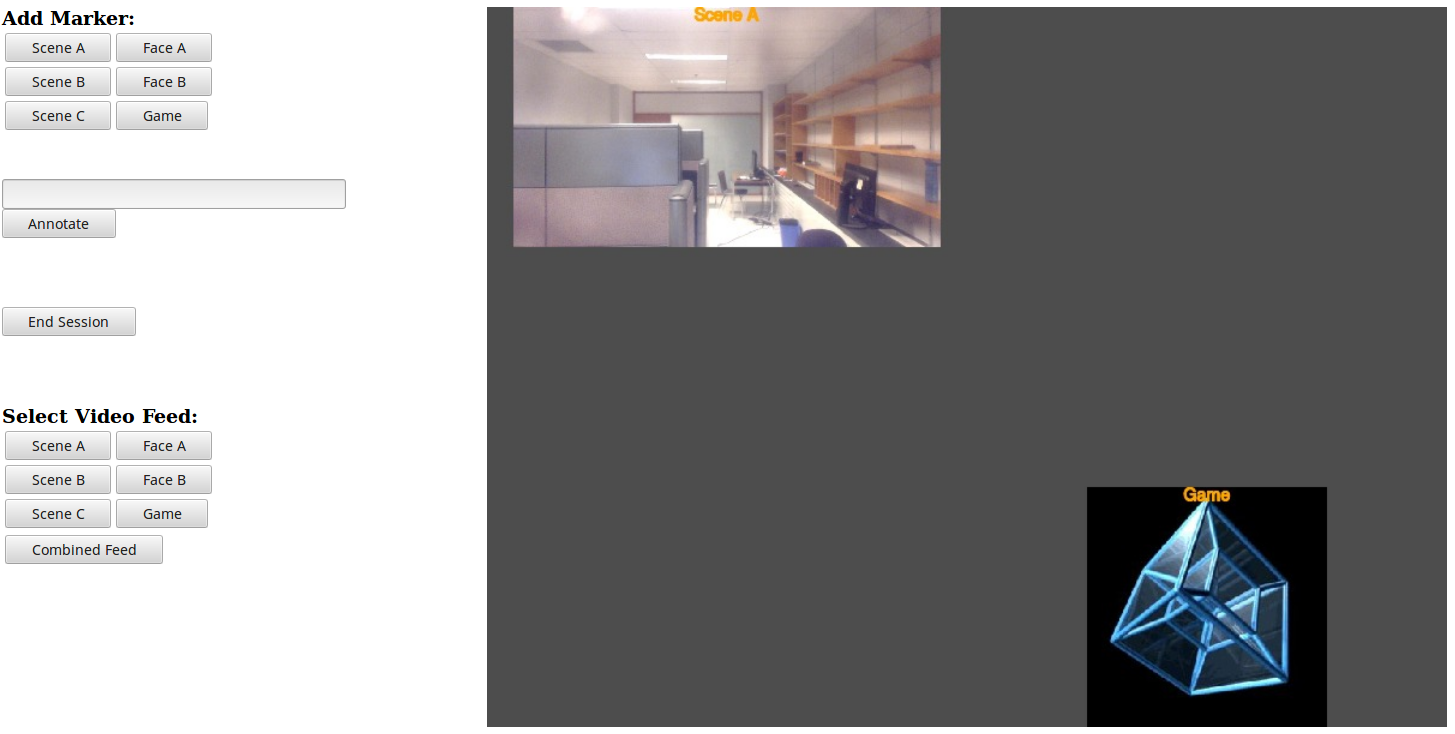
\includegraphics[width=0.95\textwidth]{pics-gui/gui-monitor.png}
\end{center}
\caption{Monitoring screen.}\label{fig-gui-monitor}
\end{figure}

% FIXME - Annotate the image.

The monitoring screen is used to view the progress of a capture session that
is underway, and to add event markers to the log file for this session.

The ``Add Marker'' buttons produce timestamped log entries indicating
events of interest in their respective video feeds.

The ``Annotate'' button produces a timestamped log entry containing
user-supplied text.

The ``End Session'' button stops video capture, closes the log file, and
switches to the repository browser screen. This may alternatively be done
by raising the ``stop capture'' TTL line.

The ``Select Video Feed'' buttons replace the combined image with the raw
video frames from the selected feed. This is usually better-quality and 
faster than the combined feed. The ``Combined Feed'' button returns to the
composite feed.

\section{Repository Browser}
\label{gui-repo}

\begin{figure}[h]
\begin{center}
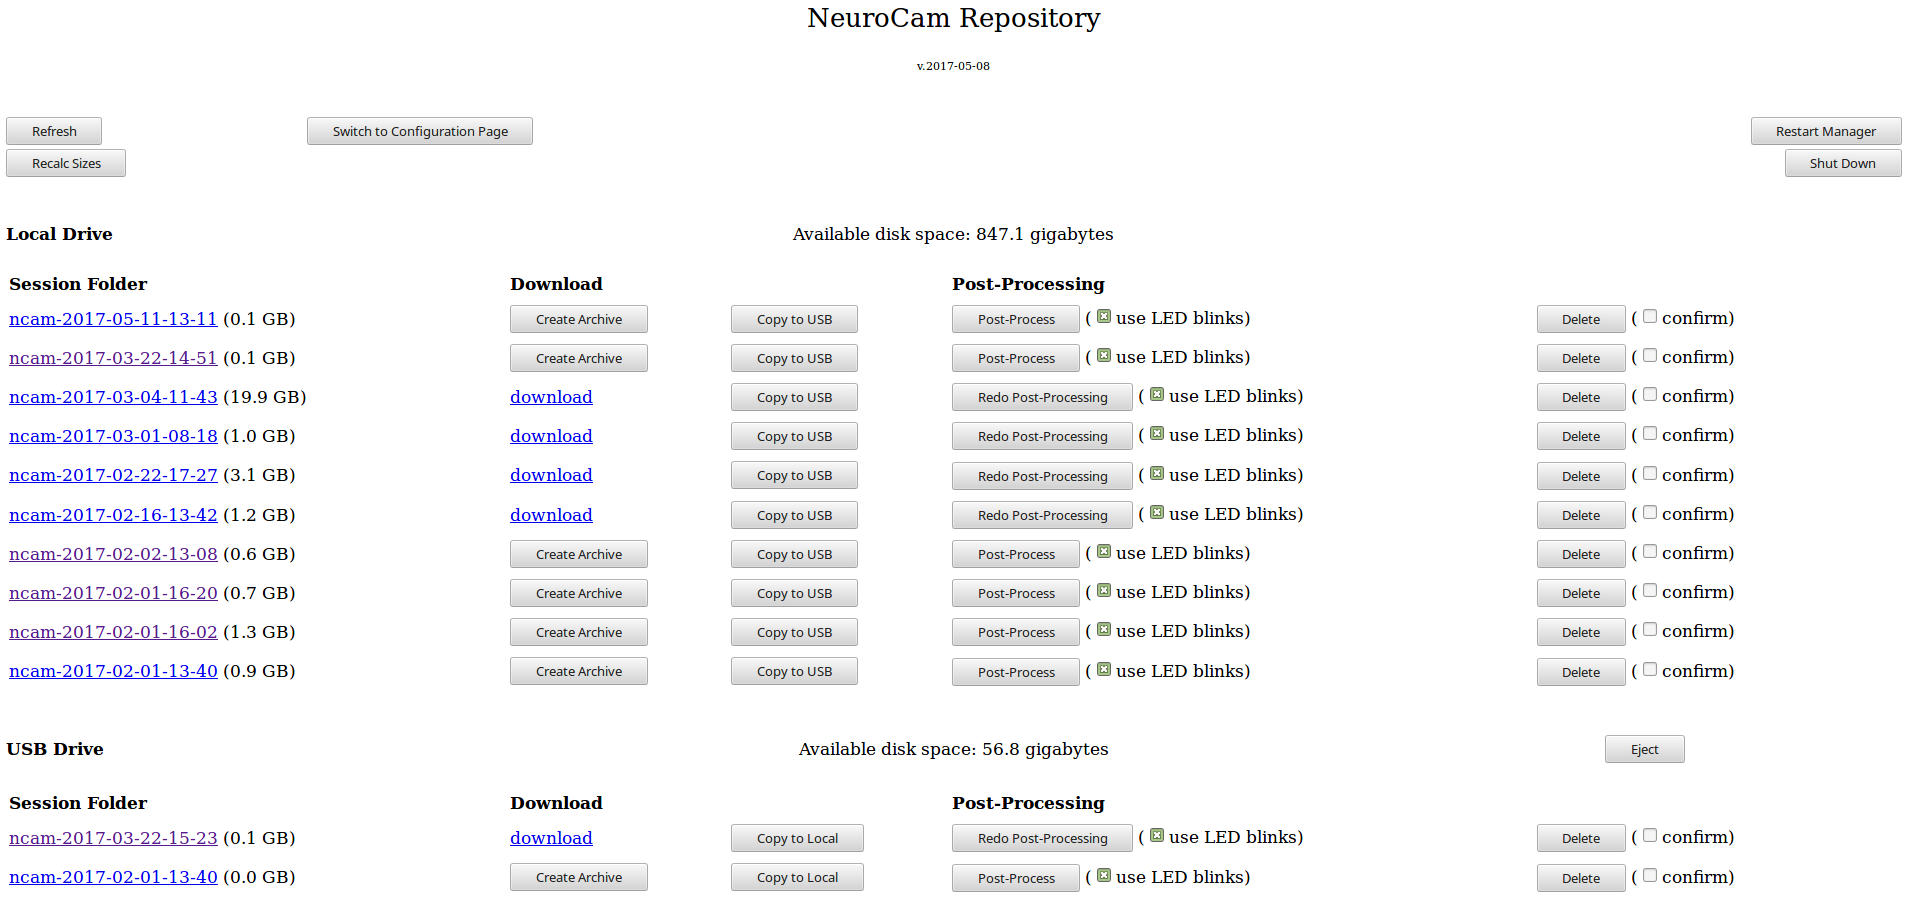
\includegraphics[width=0.95\textwidth]{pics-gui/gui-browser.png}
\end{center}
\caption{Repository browser.}\label{fig-gui-repo}
\end{figure}

% FIXME - Annotate the image.

The repository browser is used to inspect the data files produced by
past sessions, to perform post-processing of session data, and to download
and transfer packaged session data. Old sessions may also be deleted to free 
up disk space.

The ``Session Folder'' column lists sessions within the repository. Clicking
on a session name opens that session's directory in a new window. Files may
be individually inspected and downloaded via that window. See Chapter 
\ref{repo} for a description of the repository folder contents.

The ``Download'' column contains a link to a ``.tar'' archive containing
a session's entire directory tree. This is intended to provide an easy way
to transfer a session's data over the network. The archive is created using 
the ``Create Archive'' button. If post-processing has been performed, the 
archive includes the post-processed files. \textbf{NOTE:} The archive file 
is large. Check that there is sufficient free space before creating it.

The ``Copy to USB'' and ``Copy to Local'' buttons create duplicates of their
session folders on a USB-attached drive and on the local drive, respectively.
\textbf{NOTE:} These may instead be named ``Move to USB'' and ``Move to 
Local'', depending on settings. ``Move'' deletes the original folder, while
``Copy'' leaves it in place.

The ``Post-Processing'' button triggers several operations on a session 
folder. If the ``use LED blinks'' checkbox is set, video timestamps are
synchronized with each other using flashes of the infrared LEDs. A new log
file is saved with these adjusted timestamps. After synchronization, a
``Composite'' video feed is created, arranged in the same manner as the 
monitoring feed but at higher resolution and with full frame rate. A new log
file is saved with composite feed frame events added. Finally, movie files
of all video feeds are created for easy preview/playback.
\textbf{NOTE:} Post-processing operations take a lot of time on the local
drive (a solid-state drive), and even longer on magnetic platter or flash
drives.

\fixme{Benchmark post-processing. How long does processing an hour of
five-camera-plus-game footage take?}

The ``Delete'' buttons allow individual session folders (and their archives)
to be removed. This cannot be undone; to prevent accidental deletion, the
corresponding ``confirm'' checkbox must be checked before pressing the
``Delete'' button. Deleting old sessions will need to be performed frequently
in order to free up disk space.

The ``Eject'' button unmounts an external drive so that it can be safely
removed. \textbf{NOTE:} Writing data to an external drive can take a while,
so please wait until the NeuroCam indicates that it is safe for the drive
to be removed.

The ``Refresh'' button re-scans the repository directory for new sessions.

The ``Recalc Sizes'' button recomputes metadata for all session folders.
\textbf{NOTE:} This can take a while, as each session may contain millions
of files.

The ``Switch to Configuration Page'' button changes to the configuration
screen, so that the next capture session may be set up.

The ``Restart Manager'' button forcibly restarts the NeuroCam software. This
allows recovery if any part of the NeuroCam software stops behaving correctly.
This is also needed if performing a software update without restarting the
NeuroCam machine.

The ``Shut Down'' button turns off the NeuroCam computer.

%
% This is the end of the file.
